\documentclass[11pt, a4paper]{article}
\usepackage[utf8]{inputenc}
\usepackage[left=2cm, right=2cm, top=2.5cm, bottom=2.0cm]{geometry}
\usepackage{amsmath, amssymb, amsthm}
\usepackage[english]{babel}
\usepackage{graphicx}
\usepackage[font={small,it}]{caption}
\graphicspath{ {figures/} }
\usepackage{url}
\usepackage{appendix}
\usepackage{float}
\usepackage[bottom]{footmisc}
\usepackage{titling}
\setlength{\droptitle}{-10em}  

\title{ \huge Artificial neural networks \\ 
  { \large Assignment 1: Supervised learning and generalization }}
\author{
        Lood, Cédric \\
        \small Master of Bioinformatics
}

\begin{document}
\maketitle
%\tableofcontents

\section{Context}

Artificial neural networks that have at least 1 hidden layer have the
property of being universal
approximator\cite{hornik1989multilayer,leshno1993multilayer}. Hence,
any non-linear function can be realized using classical feedforward
multilayers networks. Here, I explore batch learning with different
training algorithms and compare their yields in terms of performance,
training time, and generalization. For the sake of illustration, I
used the underlying, known function $f(x)=e(-x^2)sin(10x)$ to generate
the dataset for batch supervised learning. The architecture of the
neural network consists of 10 hidden units with sigmoid transfer
function, 1 input, and 1 output (linear).

\section{Noise-free learning}

The function $f(x)$ was learned using noiseless datapoints over the
range $[-\pi;\pi]$ by interval of $\delta x = 0.1$. The training
algorithm selected are the ones reviewed during the lecture. Their
relative performances can be appreciated by looking at the figure
\ref{fig:trainnl}. On the left-hand side, the approximation of the
different learning schemes after 100 epochs. On the right-hand side,
the training error as it evolve during training.

\begin{figure}[H]
  % \centering
  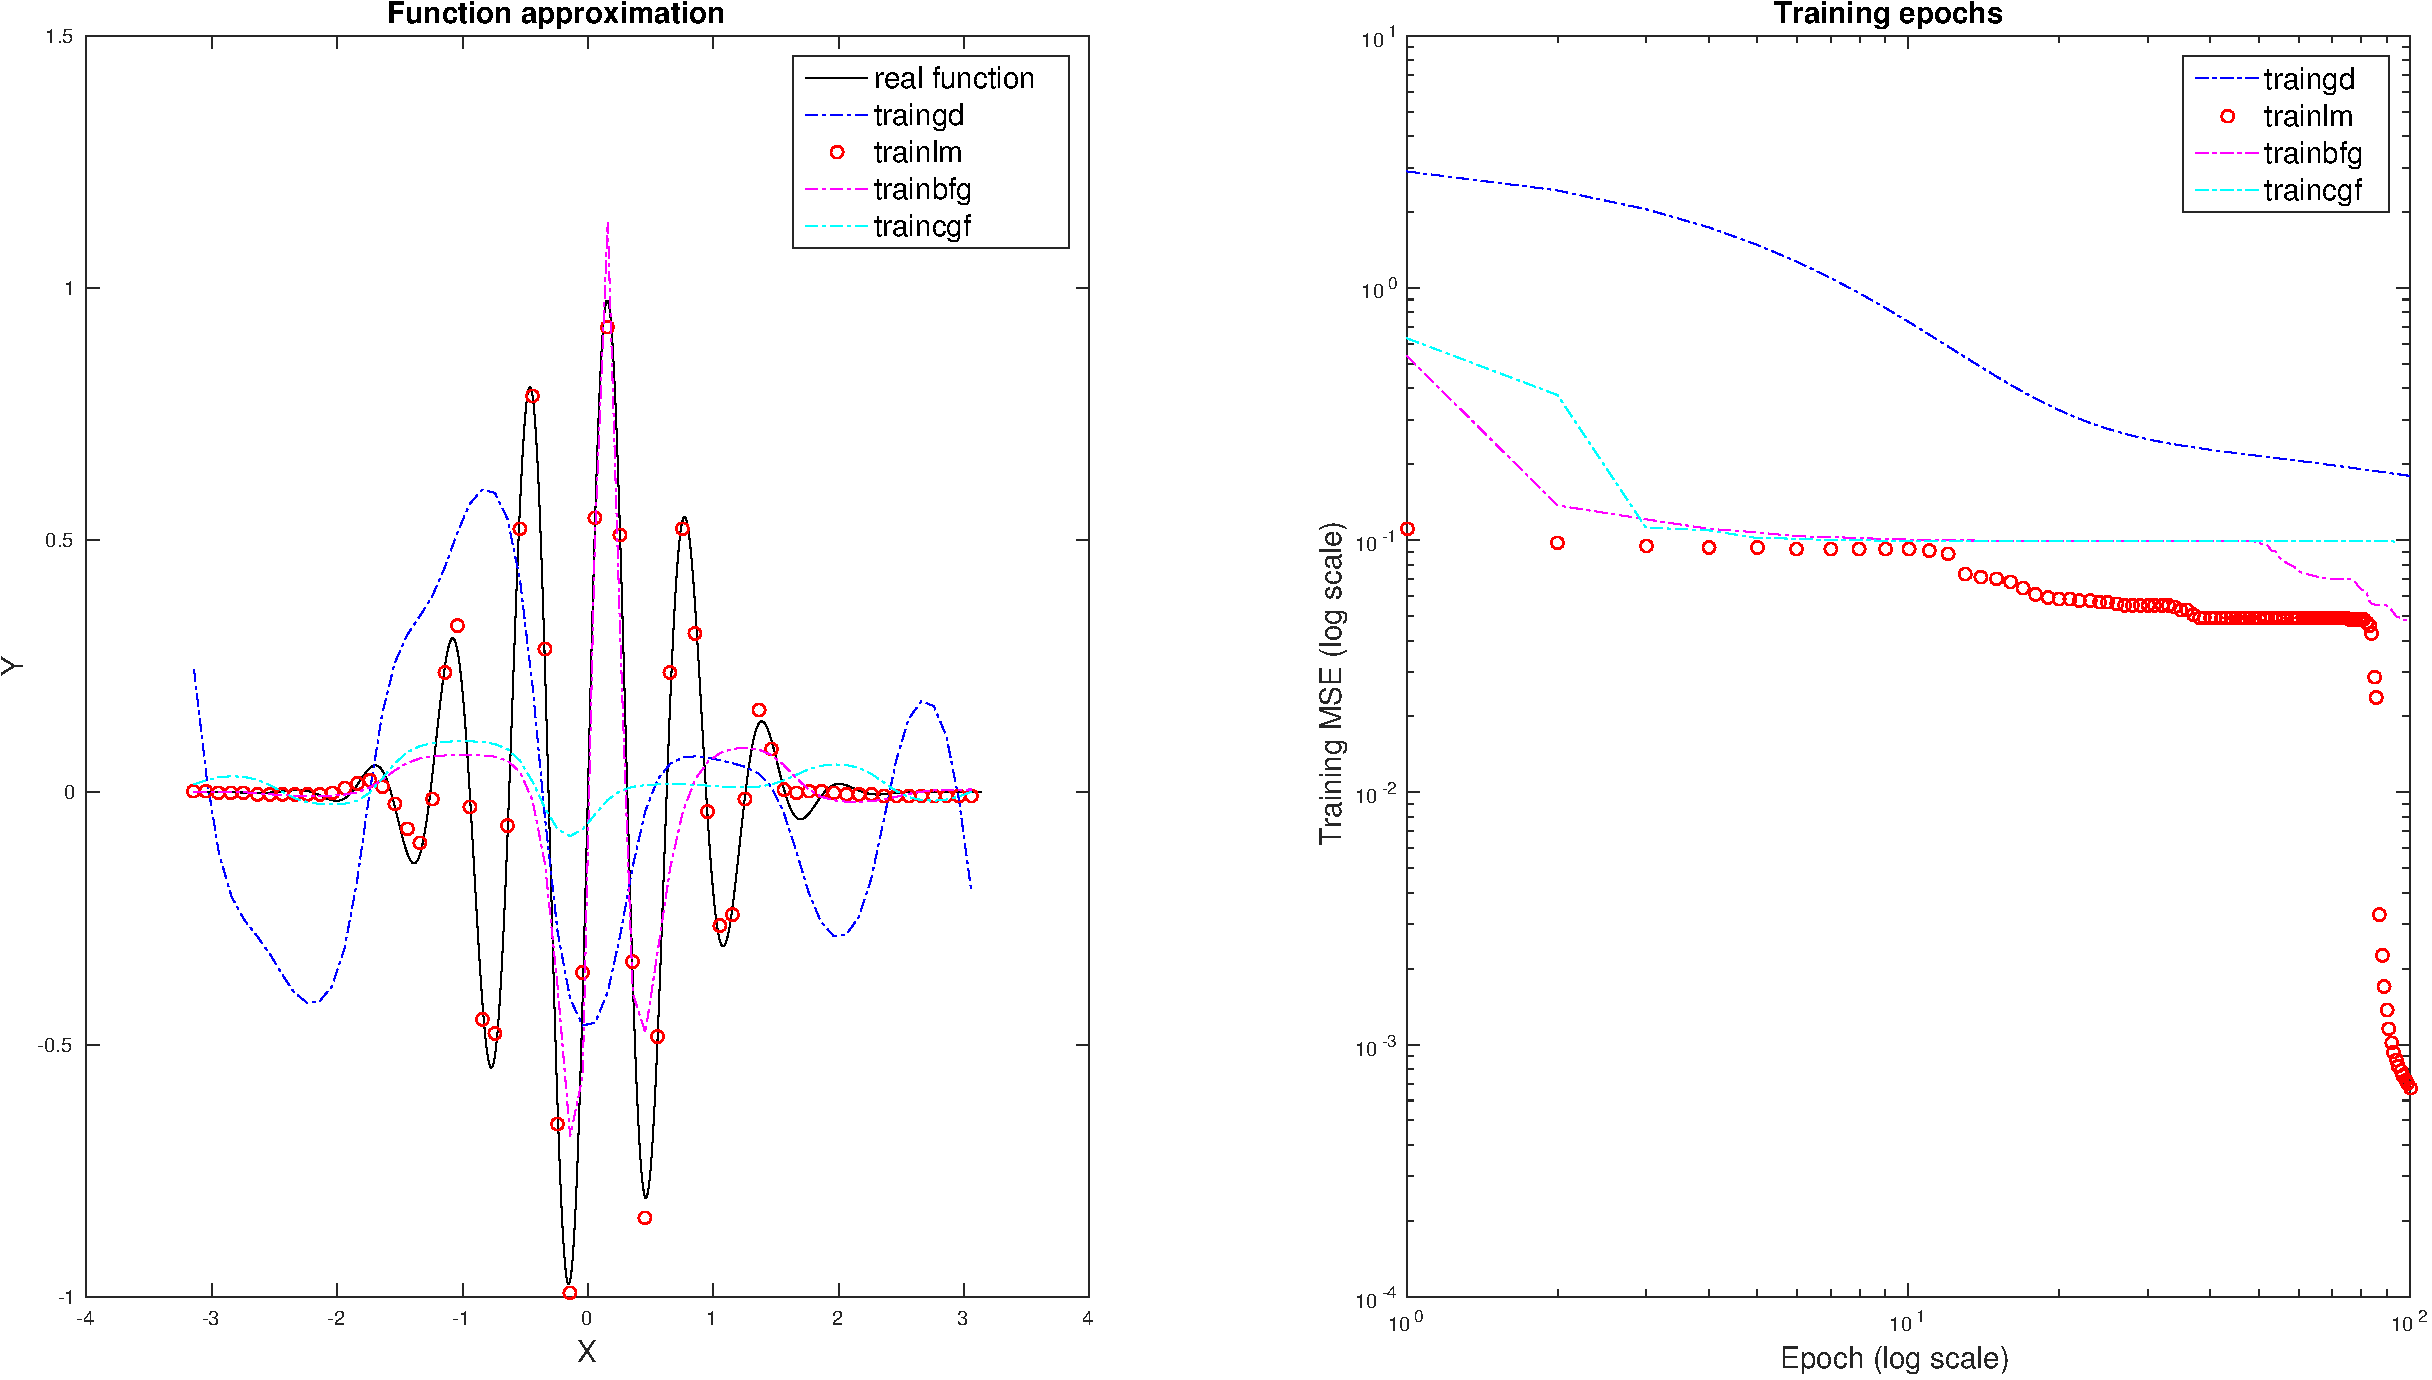
\includegraphics[scale=.43]{training_performance.pdf}
  \caption{Training performance}
  \label{fig:trainnl}
\end{figure}

\begin{description}
\item [traingd] is the gradient descent algorithm. Its performance
  were rather terrible in terms of function approximation. The
  implementation details are simple, but it suffers from slow
  convergence.
\item [trainlm] was the best performer overall with the different
  functions I tried to approximate. The algorithm ressembles the
  Newton method but has an extra-term that enables solving otherwise
  ill-conditioned problems.
\item [trainbfg] is a quasi-Newton method. This algorithm avoids the
  computation of the Hessian matrix, and works instead with an
  approximation, sparing CPU cycles.
\item [traincgf] is a conjugate gradient approach, which can be really
  useful when dealing with networks that have a lot of hidden neurons
  and/or interconnections. This algorithm avoids storing the Hessian
  matrix, sparing the RAM needed otherwise to store potentially huge
  matrices.
\end{description}

\section{Learning in noisy setting}

For this section, I worked with a slightly easier function
$f(x)=x^3-11x+2$. To simulate the presence of noise in the dataset, I
chose to add a normally distributed noise:
$f_{noisy}(x)=f(x)+N(0,1)$. The gradient descent algorithms was
replaced with gradient descent with momentum (\emph{traingda}) as the
variance in the function lead to an infinite gradient (a solution
would have been to normalize the function and work with z-scores)

Given that we work with a synthetic dataset, we can work out the true
mean square error between the underlying function and the model
trained on the noisy data. I tried to get a sense for the impact of
the amount of training cycles (Epochs) on the MSE (fixed number of
neurons). There seems to be much fluctuation. Function estimation
after $10^3$ epochs is also reported on the graph, as one can see, the
\emph{trainlm} approach does seem to overfit the data more. An obvious
approach to avoid overfitting in a real case dataset would be to use
crossvalidation to select the correct amount of neurons and epochs.

\begin{figure}[H]
  % \centering
  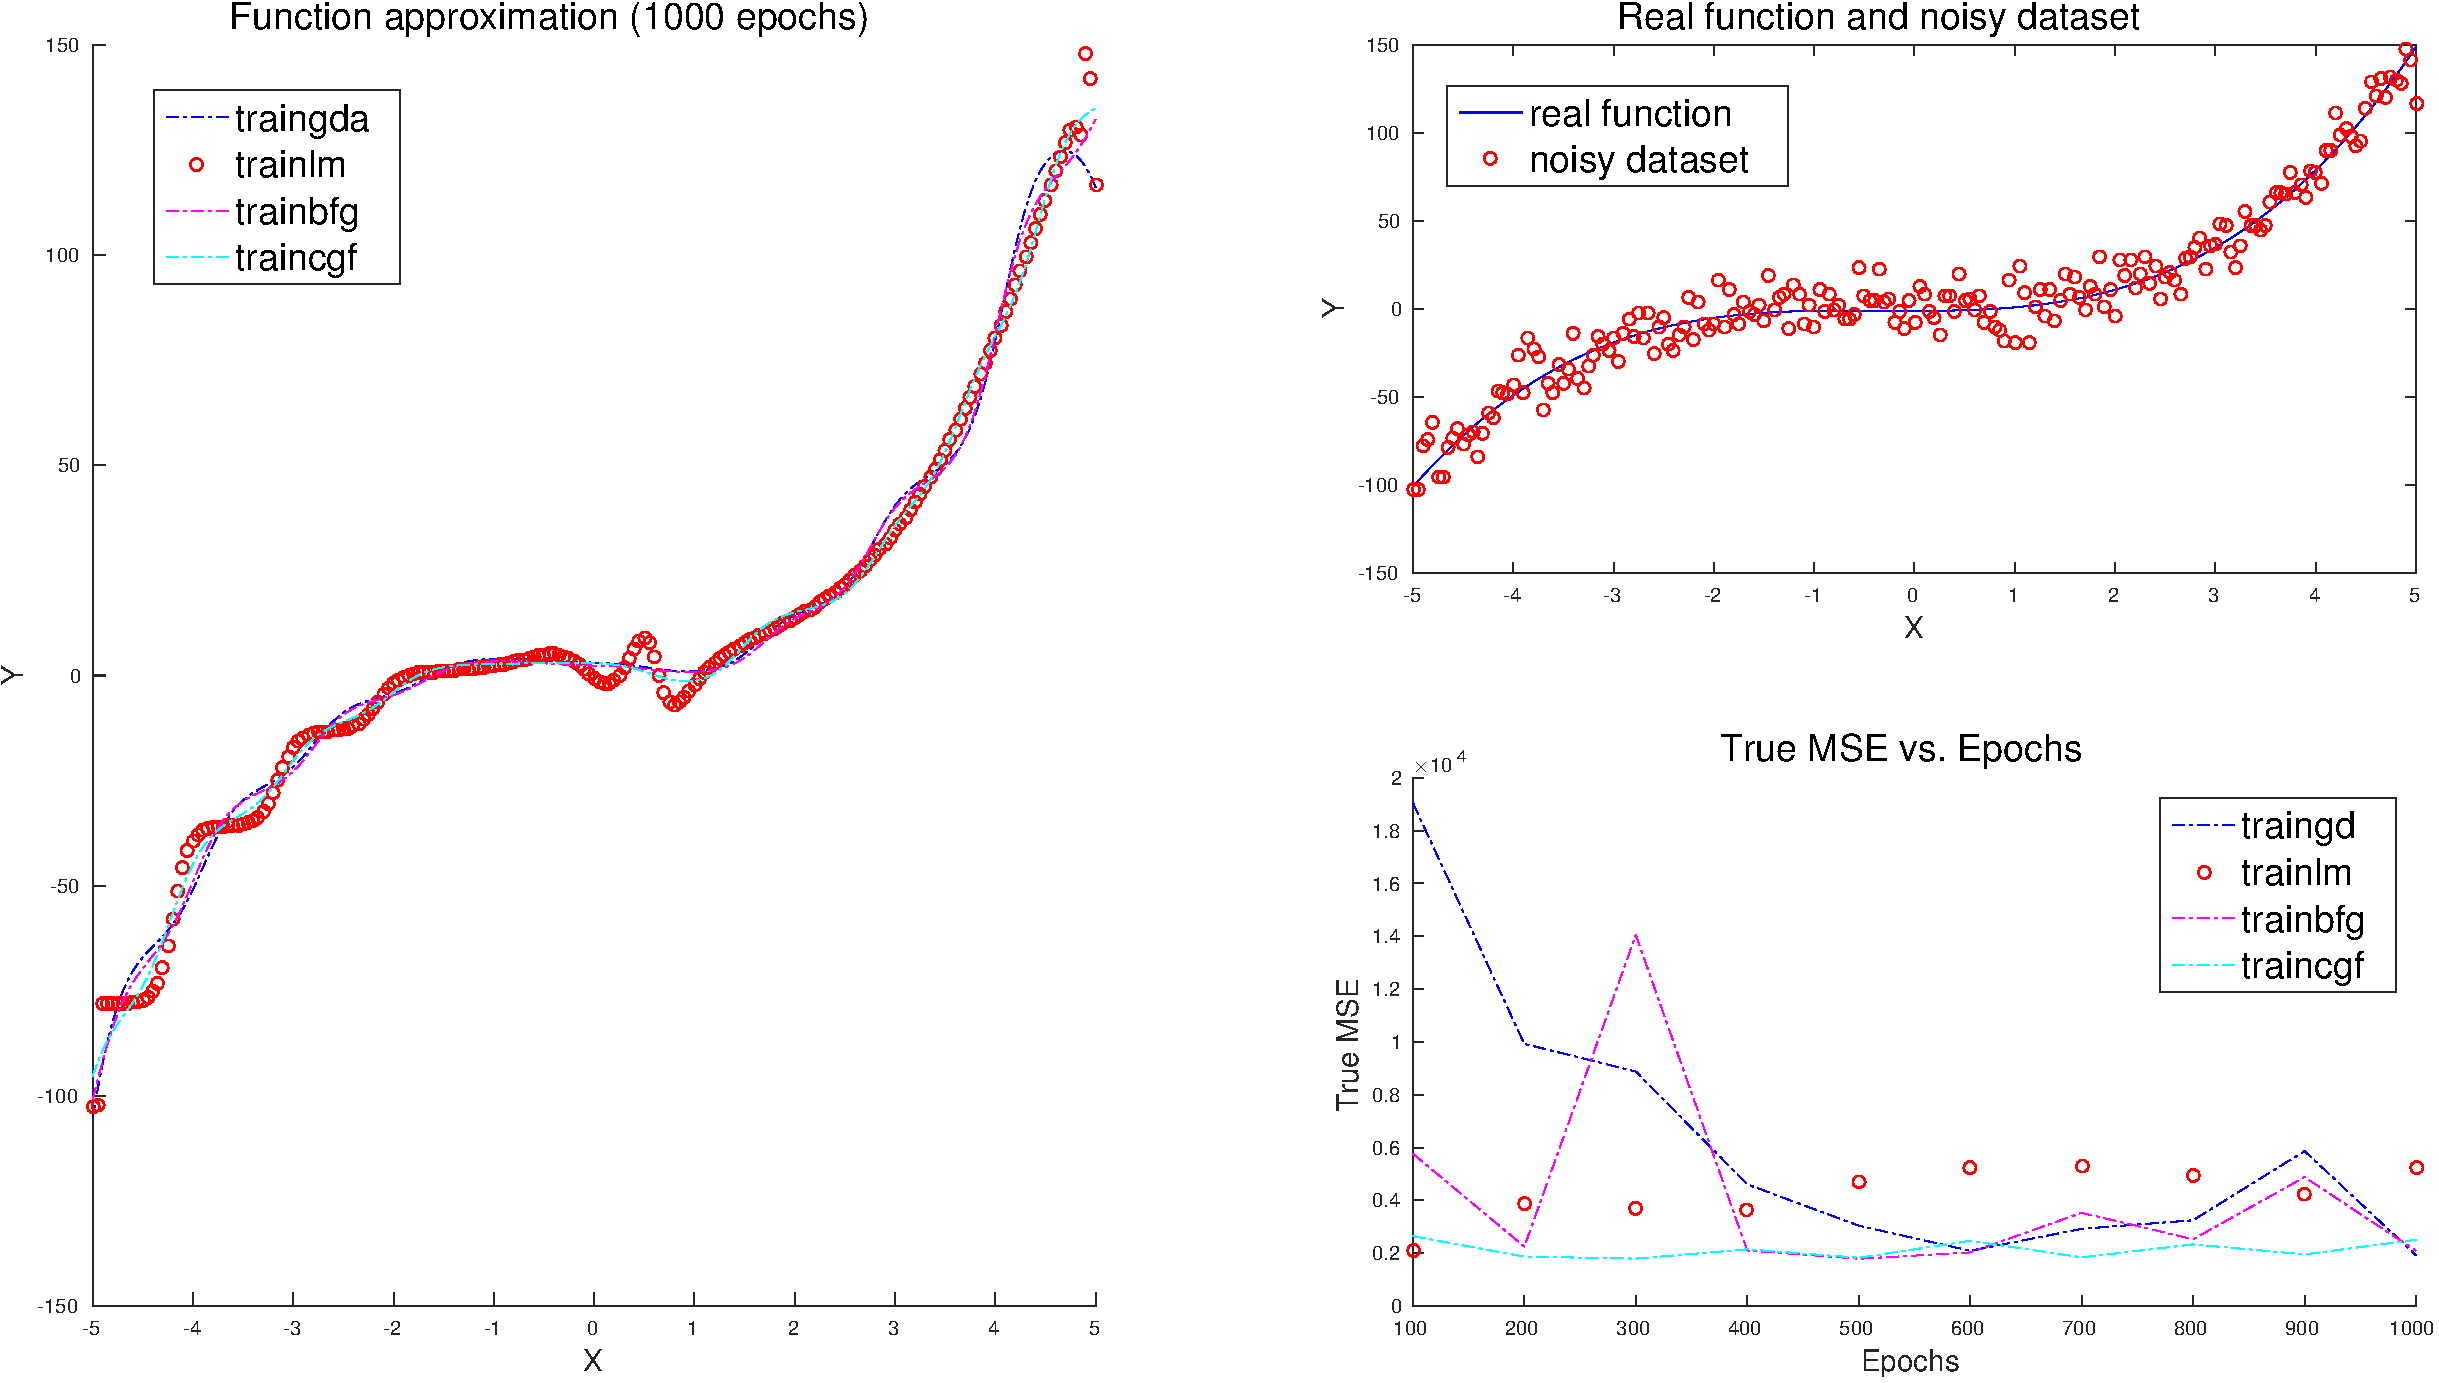
\includegraphics[scale=.40]{ffnn_noisy_testmse.pdf}
  \caption{Example of overfitting in noisy dataset}  
  \label{fig:trainnoise}
\end{figure}

{\footnotesize
\bibliographystyle{ieeetr} 
\bibliography{bib-db}}

\end{document}
